\newpage

\section{Jakub Łabuz}

\subsection{Wyrażenie matematyczne}
Spójrzmy na taką granicę:
\[ \lim_{n\to\infty} \sin^n \frac{n+1}{n} = 1\]

\subsection{Piękne zdjęcie pięknego miejsca}
\begin{figure}[h]
    \centering
    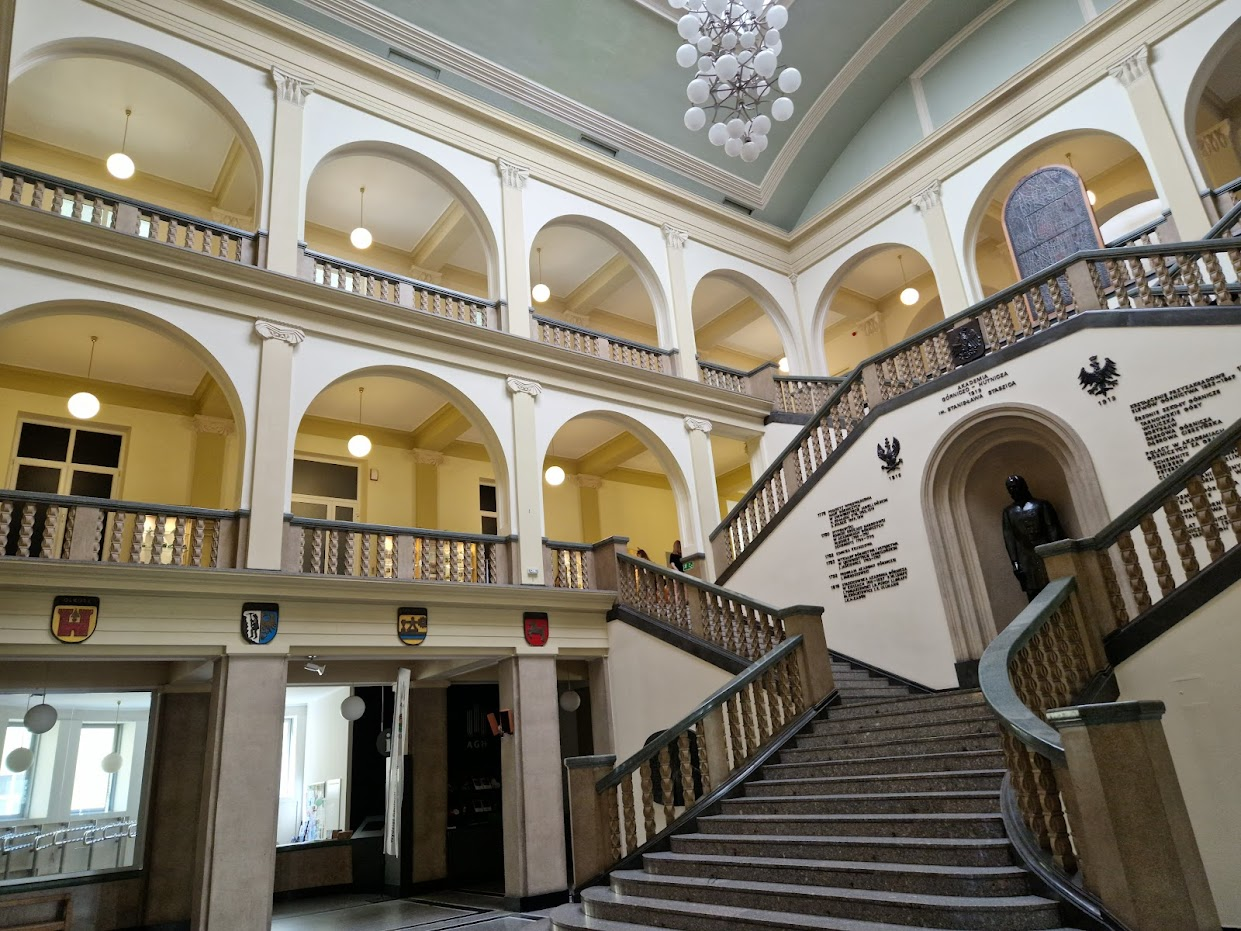
\includegraphics[scale=0.3]{pictures/obrJŁ/1}
    \caption{Wnętrze gmachu głównego AGH}
    \label{fig:agh}
\end{figure}


\newpage
\subsection{Tabela}
Zagłębmy się w tegoroczne statystyki maturalne:
% Please add the following required packages to your document preamble:
% \usepackage[table,xcdraw]{xcolor}
% Beamer presentation requires \usepackage{colortbl} instead of \usepackage[table,xcdraw]{xcolor}
\begin{table}[H]
\begin{tabular}{l|ll|ll|ll|}
\cline{2-7}
 & \multicolumn{2}{l|}{{\color[HTML]{009901} Wszyscy zdający}} & \multicolumn{2}{c|}{{\color[HTML]{6200C9} \begin{tabular}[c]{@{}c@{}}absolwenci liceum\\ (nowa formuła)\end{tabular}}} & \multicolumn{2}{c|}{{\color[HTML]{CD9934} \begin{tabular}[c]{@{}c@{}}absolwenci technikum,\\ szkoły artystycznej\\ oraz szkoły branżowej\\ II stopnia\\ (stara formuła)\end{tabular}}} \\ \hline
\multicolumn{1}{|l|}{liczba maturzystów:} & \multicolumn{1}{l|}{{\color[HTML]{009901} 254 610}} & {\color[HTML]{009901} 100\%} & \multicolumn{1}{l|}{{\color[HTML]{6200C9} 151 717}} & {\color[HTML]{6200C9} 100\%} & \multicolumn{1}{l|}{{\color[HTML]{CD9934} 102 893}} & {\color[HTML]{CD9934} 100\%} \\ \hline
\multicolumn{1}{|l|}{ci, którzy zdali maturę:} & \multicolumn{1}{l|}{{\color[HTML]{009901} 227 440}} & {\color[HTML]{009901} 89,3\%} & \multicolumn{1}{l|}{{\color[HTML]{6200C9} 143 564}} & {\color[HTML]{6200C9} 94,6\%} & \multicolumn{1}{l|}{{\color[HTML]{CD9934} 83 876}} & {\color[HTML]{CD9934} 81,5\%} \\ \hline
\multicolumn{1}{|l|}{ci, którzy nie zdali:} & \multicolumn{1}{l|}{{\color[HTML]{009901} 27 170}} & {\color[HTML]{009901} 10,7\%} & \multicolumn{1}{l|}{{\color[HTML]{6200C9} 8 153}} & {\color[HTML]{6200C9} 5,4\%} & \multicolumn{1}{l|}{{\color[HTML]{CD9934} 19 017}} & {\color[HTML]{CD9934} 18,5\%} \\ \hline
\end{tabular}
\caption{Zdawalność matury 2023}
\label{tab:matura2023}
\end{table}

\subsection{Lista}
Aktorzy grający Jamesa Bonda w produkcjach oficjalnych w kolejności występowania w filmach:
\begin{enumerate}
    \item Sean Connery (1962-1967, 5 filmów)
    \item George Lazenby (1969, 1 film)
    \item Sean Connery (1971, powrót na jeden film - w sumie 6)
    \item Roger Moore (1973-1985, 7 filmów)
    \item Timothy Dalton (1987-1989, 2 filmy)
    \item Pierce Brosnan (1995-2002, 4 filmy)
    \item Daniel Craig (2006-2021, 5 filmów)
\end{enumerate}
Brytyjskiego agenta w produkcjach niezależnych zagrali:
\begin{itemize}
    \item[*] Barry Nelson (1954, film telewizyjny)
    \item[*] David Niven (1967, 1 film - parodia)
    \item[*] Sean Connery (1983, 1 film)
\end{itemize}

\subsection{Tekst}

\par
W PEWNEJ NORZE ZIEMNEJ MIESZKAŁ SOBIE PEWIEN hobbit. Nie była to szkaradna, brudna, wilgotna nora, rojąca się od robaków i cuchnąca błotem, ani też sucha, naga, piaszczysta nora bez stołka, na którym by można usiąść, i bez dobrze zaopatrzonej spiżarni; była to nora hobbita, a to znaczy: nora z wygodami.\par Miała drzwi doskonale okrągłe jak okienko okrętowe, pomalowane na zielono, z lśniącą, żółtą mosiężną klamką, sterczącą dokładnie pośrodku. Drzwi prowadziły do hallu, który miał kształt rury i wyglądał jak tunel: był to bardzo wygodny tunel, nie zadymiony, z boazerią na ścianach i chodnikiem na kafelkowej podłodze; nie brakowało tu politurowanych krzeseł ani mnóstwa wieszaków na kapelusze i płaszcze, bo hobbit bardzo lubił gości. Tunel wił się w skrętach, wił się i wił, wdrażając się głęboko, choć wcale nie prostą drogą, we wnętrze pagórka – a raczej: Pagórka, bo tak go nazywano w promieniu wielu mil – a mnóstwo okrągłych drzwiczek otwierało się to po jednej, to po drugiej jego stronie. Hobbici nie uznają schodów. Sypialnie, łazienki, piwnice, spiżarnie (mnóstwo spiżarni!), garderoby (hobbit miał kilka pokoi przeznaczonych wyłącznie na ubrania), kuchnie, jadalnie – wszystko mieściło się na tym samym piętrze, a nawet wzdłuż tego samego korytarza. Najparadniejsze pokoje znajdowały się z lewej strony (patrząc od wejścia), ponieważ tylko te miały okna, głęboko osadzone, okrągłe okna z widokiem na ogród, a dalej na łąki, zbiegające w dół ku rzece.\par
\begin{flushright}
J. R. R. Tolkien, \textit{Hobbit, czyli tam i z powrotem}
\end{flushright}
\par
\begingroup
    \centering
    Być może nora Hobbita była tak piękna jak miejsce ukazane wcześniej \textbf{na zdjęciu \ref{fig:agh} na stronie \pageref{fig:agh}} \Huge{\smiley{}} %$\ddot\smile$
    \normalsize
    O wynikach \textbf{w tabeli \ref{tab:matura2023} na stronie \pageref{tab:matura2023}} nie wspominam, bo Hobbici najpewniej matury nie mieli... \Huge{\frownie{}}
\endgroup
\subsection{Zmiany lokalne w repozytorium PyPou-latex}
\begin{itemize}
	\item Te punkciki
	\item dodane zostały
	\item za pomocą nano
	\item w git bash'u lokalnie
	\item w celu pobrania zmian lokalnych na overleafa online 
\newpage
